%!xelatex = 'xelatex --halt-on-error %O %S'

\documentclass{buaaemp}
\begin{document}

% 标题,作者
\emptitle{题目一般不超过20个字}
\empauthor{智朝晖}{张高龙}

% 奇数页页眉 % 请在这里写出第一作者以及论文题目
\fancyhead[CO]{{\footnotesize 智朝晖: 某实验的实验报告}}


%%%%%%%%%%%%%%%%%%%%%%%%%%%%%%%%%%%%%%%%%%%%%%%%%%%%%%%%%%%%%%%%
% 关键词 摘要 首页脚注
%%%%%%%%关键词
\Keyword{关键词, 很关键的词, 十分关键的词, 有一些关键的词, 大关键词}
\twocolumn[
\begin{@twocolumnfalse}
\maketitle

%%%%%%%%摘要
\begin{empAbstract}
摘要内容,小五号宋体,不超过500字。简要概述主要实验内容和结果。要求:论文的基本信息和要点都应该出现在摘要里;使用标准精确的词汇和语言,清晰紧凑地概述客观事实;摘要的整体结构严谨、思路清楚,基本素材组织合理。英文摘要与中文内容一致。英文摘要须与中文内容一致,被动语态、现在时。字号为小五New Times Roman。论文的中、英文摘要是国内外数据库收录的主要内容,所以摘要的内容直接影响到该论文能否被收录及收录后被引用的情况,作者应给予高度重视。关键词为经过规范化处理的词语或短语,数量一般为3~5个。同一篇文章的中英文关键词的内容和顺序应一致。
\end{empAbstract}

%%%%%%%%首页角注,依次为实验时间、报告时间、学号、email
\empfirstfoot{2022-09-15}{2022-9-16}{20377365}{20377365@buaa.edu.cn}
\end{@twocolumnfalse}
]
%%%%%%%%!首页角注可能与正文重叠,请通过调整正文中第一页的\enlargethispage{-3.3cm}位置手动校准正文底部位置:
%%%%%%%%%%%%%%%%%%%%%%%%%%%%%%%%%%%%%%%%%%%%%%%%%%%%%%%%%%%%%%%%
%  正文由此开始
\wuhao 
%  分栏开始

\section{引~~言}
正文内容,五号宋体:引言应简要说明所做实验的背景和意义,介绍相关领域内前人所做的工作和研究的概况,以及本文着力解决的问题;本文的主要研究内容和结果概述。

行文应言简意赅,不要重复摘要和解释摘要,防止吹嘘自己和贬低别人,避免宣传性的用语,尽量不要出现图表。引言中关于目前与本实验有关领域的研究进展和应用,最好自己上网查阅一两篇综述文献做大概的了解,查文献并对文献总结是做科研必备的基本功,希望在近物实验中有所体验。文中引用的结论性文字要标注参考文献,须加方括号,一般置于右上角。如\cite{钱建强2016近代物理实验}

注意学术诚信,正文各层次标题一律用阿拉伯数字连续编码,并左顶格书写,序码之后空一个汉字间距接写标题。
\section{原~~理}

\section{实~~验}
正文内容:正文文字五号宋体。
\enlargethispage{-3.3cm}
简要介绍用什么型号的实验仪器在什么样的实验条件下做了哪些实验内容,这些内容是通过什么实验方法来实现的等。
实验内容不是指实验操作步骤,实验部分写作重点是实验方法和实验条件,自己概括叙述,不要照抄讲义。
实验部分写作举例:用莱宝X射线衍射仪(实验仪器)测量NaCl单晶的晶格常数(内容),所用x射线为Mo靶产生的两条特征谱线,x射线管电压和电流分别为35kV、1mA(实验条件),用联动耦合方式测量4-25度范围内NaCl单晶的衍射谱,根据衍射峰的位置由布拉格衍射公式计算其晶格常数(实验方法)。


其他实验的写法也是如此,不必写具体的仪器细节,测量方法也不是操作步骤,而是实验方法。

\subsection{二级标题}
如果实验内容很多,彼此之间又相互独立,可以用二级标题的形式分开写。

\subsection{二级标题}
正文内容正文文字五号宋体正文内容正文文字五号宋体正文内容正文文字五号宋体正文内容正文文字五号宋体正文内容正文文字五号宋体正文内容正文文字五号宋体正文内容正文文字五号宋体正文内容。

\section{实验结果与分析}
一般先给出实验条件、现象和实验结果,然后用学过的物理理论结合实验条件做出合理的分析和解释。

实验数据及处理结果在报告中以图或表形式给出,并对图、表所反映的现象或物理规律做出具体说明和解释。图、表格式规范,大小适中。

分析讨论影响实验结果的因素,改进方法等


\subsubsection{三级标题}

\subsection{报告中公式、字母的规范写法}
公式全文统一编号,如公式为
\begin{equation}\label{EQ1}
\frac{\partial u}{\partial x}+\frac{\partial v}{\partial y}+\frac{\partial w}{\partial z}=0
\end{equation}
式中,$u$是××××(单位);$v$是×××(单位);$w$是××(单位)。

对于公式,应全文统一连续编号,如式\eqref{EQ1}……一般情况下,需要引用的或重要的公式才编号。在文中引用时,用“式(编号)”表示。
后文不再提及的,可以不编号。如
\begin{equation*}
1 + 1 + 3 = 5
\end{equation*}

对于公式中首次出现的量的符号,按照其在式中出现的顺序,用准确、简洁的语句对其进行逐一解释。公式中变量应尽量避免复合上下角标的使用;尽量少用3层关系的上下标,同时应尽量减少不必要的公式推导。

\subsection{报告中图的规范要求}
插图全文顺序编号。插图内容应与正文内容密切结合,每幅图前都应有相应的引出或介绍文字。图形应保证线条清晰,图形大小应适应版面要求,合理布局,图内如有标注或说明性文字时应清晰可辨。图中除了物理量符号及单位外一律用中文,同一图中的不同曲线应用不同线型表示。插图分辨率要大于600PPI。

正文文字中先见文,后见图,图号全文统一按顺序编号,如图\ref{fig:eg}所示。图中文字为6号,图线必须清晰可辨坐标轴的物理量和单位不可缺。


\begin{figure}[H]
\centering
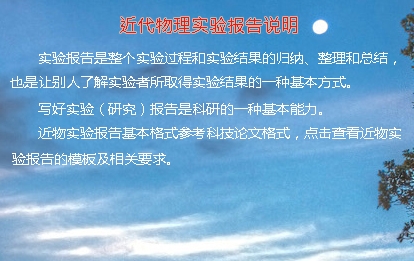
\includegraphics[width=0.8\linewidth]{./image/example.jpg}
\caption{图片示例} \label{fig:eg}
\end{figure}


\subsection{报告中表的规范}
推荐使用标准“三线表”(如表\ref{tab:eg1}所示。),内容易混淆时可加辅助线进行辅助说明。按表格在文中出现的顺序,用阿拉伯数字对其进行编号,全文顺序编号。应有相应的表题且每个表格前都应有相应的引出或介绍文字。

图、表应在文中有相应表述,即图、表的号应在文中引出,以先见文后见图、表为原则。每个图、表都必须有图名、表名,并且有编号。图号、表号应全文统一连续排列,即,应按照图1、图2……排列不应按小结编号。图片中的文字、线条应当清晰可辨,图片像素(DPI)在300以上。
表格推荐采用全线表,表头中使用量符号/量单位形式。如表\ref{tab:eg2}所示。

\begin{table}[h]
\centering
\captionnamefont{\wuhao\bf\heiti}
\captiontitlefont{\wuhao\bf\heiti}
\caption{三线表示例} \label{tab:eg1}
\liuhao
\begin{tabular}{cccc}
\toprule
{编号} &  {直径}/\si{\metre} & {静温}/\si{\kelvin} & {时间}/min\\
\midrule 
4 & 0.0349 & 268.15 & 30\\
5 & 0.01905 & 268.15 & 30\\
\bottomrule
\end{tabular}
\end{table}

\begin{table}[h]
\centering
\captionnamefont{\wuhao\bf\heiti}
\captiontitlefont{\wuhao\bf\heiti}
\caption{全线表示例} \label{tab:eg2}
\liuhao
\begin{tabular}{|c|c|c|c|c|}
\hline
U/V & I/mA & v/km·h$^{-1}$ & x/mm & p/MPa \\ \hline
\textit{12} & \textit{30} & \textit{80} & \textit{55} & \textit{110} \\ \hline
\textit{24} & \textit{34} & \textit{90} & \textit{60} & \textit{111} \\ \hline
\end{tabular}
\end{table}


\section{结~~论}
用准确、精炼的语言归纳总结使用的方法以及研究结果。

说明研究的创新价值和应用价值,包括对科技工作者的研究的价值和对产业发展的价值。

可说明自己做本实验的总结、收获和体会,对实验中发现的问题提出自己的建议。


%%%%%%%%%%%%%%%%%%%%%%%%%%%%%%%%%%%%%%%%%%%%%%%%%%%%%%%%%%%%%%%%
%  参考文献
%%%%%%%%%%%%%%%%%%%%%%%%%%%%%%%%%%%%%%%%%%%%%%%%%%%%%%%%%%%%%%%%
%  参考文献按GB/T 7714-2015《文后参考文献著录规则》的要求著录. 
%  参考文献在正文中的引用方法:\cite{bib文件条目的第一行}

\renewcommand\refname{\heiti\wuhao\centerline{参考文献}\global\def\refname{参考文献}}
\vskip 12pt

\let\OLDthebibliography\thebibliography
\renewcommand\thebibliography[1]{
  \OLDthebibliography{#1}
  \setlength{\parskip}{0pt}
  \setlength{\itemsep}{0pt plus 0.3ex}
}

{
\renewcommand{\baselinestretch}{0.9}
\liuhao
\bibliographystyle{gbt7714-numerical}
\bibliography{./TempExample}
}


\end{document}
